\documentclass[UTF8,fontset=fandol]{article}
\title{猫站小报 第 1 期}
\author{猫站小报编辑部}
\date{\today}
\usepackage{ctex}
\usepackage{indentfirst}
\setlength{\parindent}{2em}
\usepackage{listing}
\usepackage{xcolor}
\usepackage{graphicx}
\usepackage{geometry}
\geometry{left=0.3in,right=0.3in,top=0.3in,bottom=0.3in}

\begin{document}
	\maketitle
	\section{编辑部专版}
	\subsection{发刊词}
	
	\noindent
	\textbf{各位Kitten作者,Python诗人:} 
	
	编程猫社区一直以来是国内最大的少儿编程社区。2023年以来,官方的不作为使得社区比较为所,社区长期缺乏正经的技术性内容,而我们则选择一种偏传统的方式——报刊。来为编程技术留下一些思考的绿地
	
	\noindent
	\textbf{我们的小报分为四部分:}
	
	\begin{itemize}
		\item 编辑部专版 - 这里会刊登一些科技界的新闻,社区的时间,编辑部的社论
		\item 积木纪元 - 这里会刊登一些优秀的Kitten作品,被官方忽视的优秀作品我们会为你刊登
		\item 代码诗篇 - 刊登一些优秀的代码编程作品,官方并不重视Python作品,你可以在这里找到那些被忽视的代码
		\item 传火者 - 刊登一些教程类的文章,为了提升全社区的编程水平
	\end{itemize}
	
	除了第一部分外,所有部分均接受投稿,编辑的联系方式可以在每刊后记处找到。我们计划每周六在社区出刊,当然,作为一个社区项目,八分靠热情,长时间不出刊也有可能发生,你在我们在社区的帖子之下的跟帖就是对我们最大的支持。
	
	\begin{verbatim}
		print("Hello Codemao Newsletter)
	\end{verbatim}
	\pagebreak
	
	\section{积木纪元}
	\subsection{Quillay聊天室}
	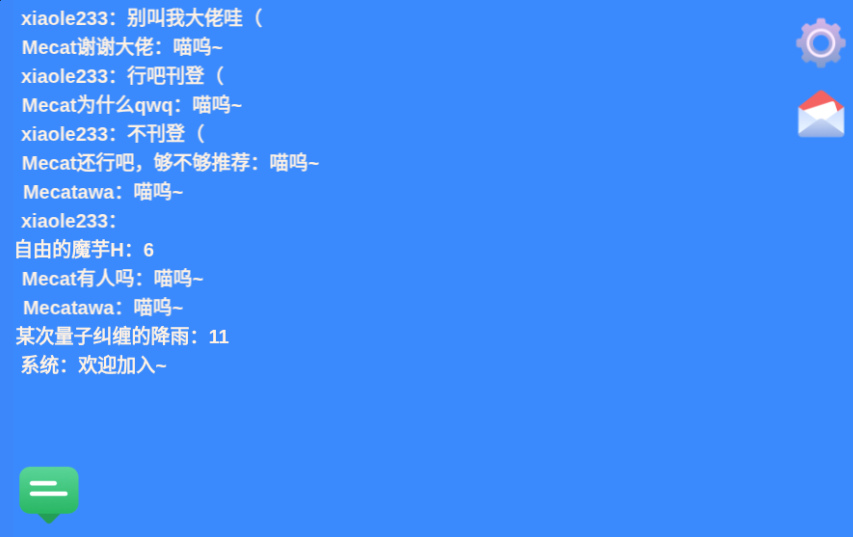
\includegraphics[width=0.5\textwidth]{assets/01/kitten-1.png}
	
	\noindent
	\textbf{作者:}Mecat \\
	\textbf{ID:}267101361 \\
	\textbf{介绍:}一个用KittenN制作的简单的聊天室,目前处于测试阶段 \\
	\textbf{编辑评:}刊登这东西的原因是Mecat的死缠烂打
	\hfill
\includegraphics[width=0.08\columnwidth]{assets/01/kitten-1-qrc.png}
	\subsection{PICKCAT斗地主}
	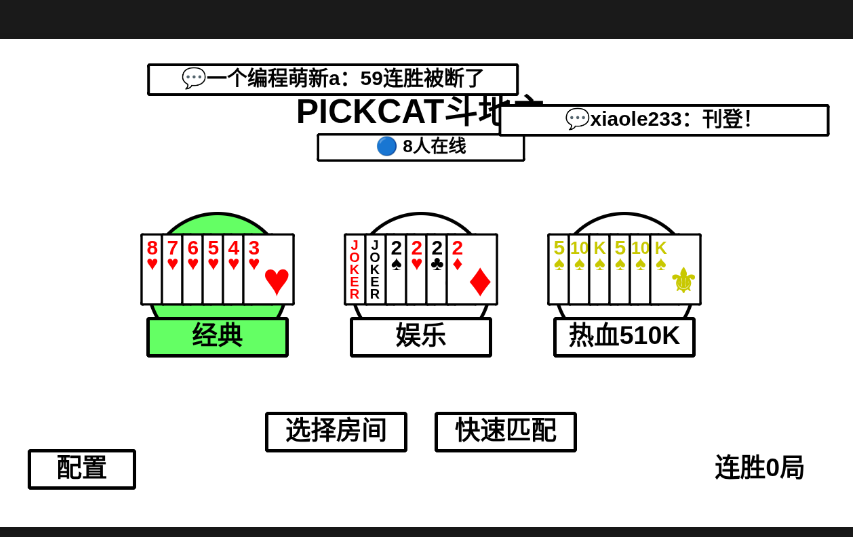
\includegraphics[width=0.5\textwidth]{assets/01/kitten-2.png}
	
	\noindent
	\textbf{作者:}钻石awa \\
	\textbf{ID:}194885331 \\
	\textbf{介绍:}一个用纯画笔公平干净的联机斗地主,据作者所说使用了1w+积木。按回车键还可以发送弹幕。\\
	\textbf{编辑评:}编辑部三缺一!
	\hfill
\includegraphics[width=0.08\columnwidth]{assets/01/kitten-2-qrc.png}
	
	\pagebreak
	\section{代码诗篇}
	\subsection{狗屁不通文章生成器}
	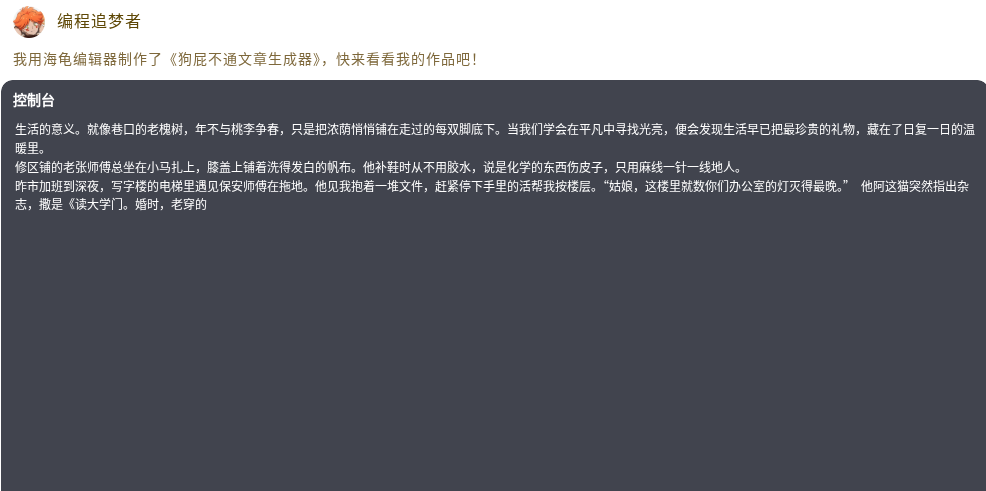
\includegraphics[width=0.5\textwidth]{assets/01/python-1.png}
	
	\noindent
	\textbf{作者:}编程追梦者 \\
	\textbf{作品ID:}276561815 \\
	\textbf{介绍:}使用Python编写的一个作文生成器,生成的作文似乎没有那么狗屁不通?\\
	\textbf{编辑评:}追梦者当时跟我说:哈哈,再也不愁作文写不出来了!应该吧(
	\hfill 
\includegraphics[width=0.08\columnwidth]{assets/01/python-1-qrc.png}
	
	\subsection{盒子IM刷屏器}
	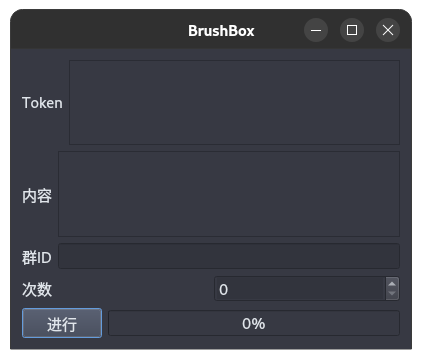
\includegraphics[width=0.5\textwidth]{assets/01/python-2.png}
	
	\noindent
	\textbf{作者:}xiaole233 \\
	\textbf{Github仓库地址:}Rov-Waff/BrushBox \\
	\textbf{介绍:}PyQt编写的一个盒子IM刷屏器,给定你的盒子IM的Token和内容就能刷屏\\
	\textbf{编辑评:}编辑卖瓜自卖自夸
	\hfill 
\includegraphics[width=0.08\columnwidth]{assets/01/python-2-qrc.png}
	
	\pagebreak
	\section{传火者}
	\begin{center}
		\zihao{-1}
		\textbf{如何看懂难以理解的代码}
		\normalsize
		供稿:虚数
	\end{center}
	
	最近有的人反馈道:
	
	imgainary\_unmber,你的3D Object Engine的代码根本看不懂啊!!!!!!
	
	那好,我就来出一个阅读逆天代码的教程
	
	首先主要就是看去除一些代码后的运行效果
	
	(也许会报错,但只需要按Ctrl+Z就行了)
	
	比方说:
	
	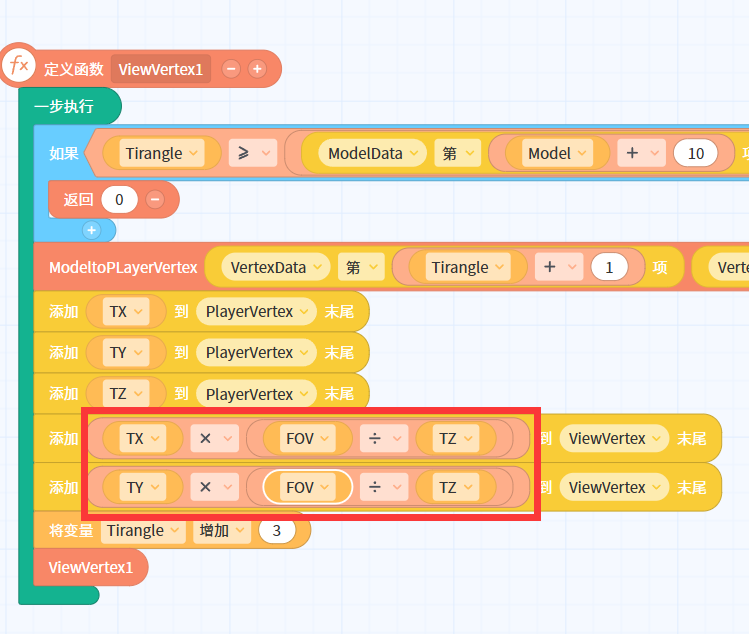
\includegraphics[width=0.5\textwidth]{assets/01/fire-1.png}
	
	我把这圈起来的地方撤掉了
	
	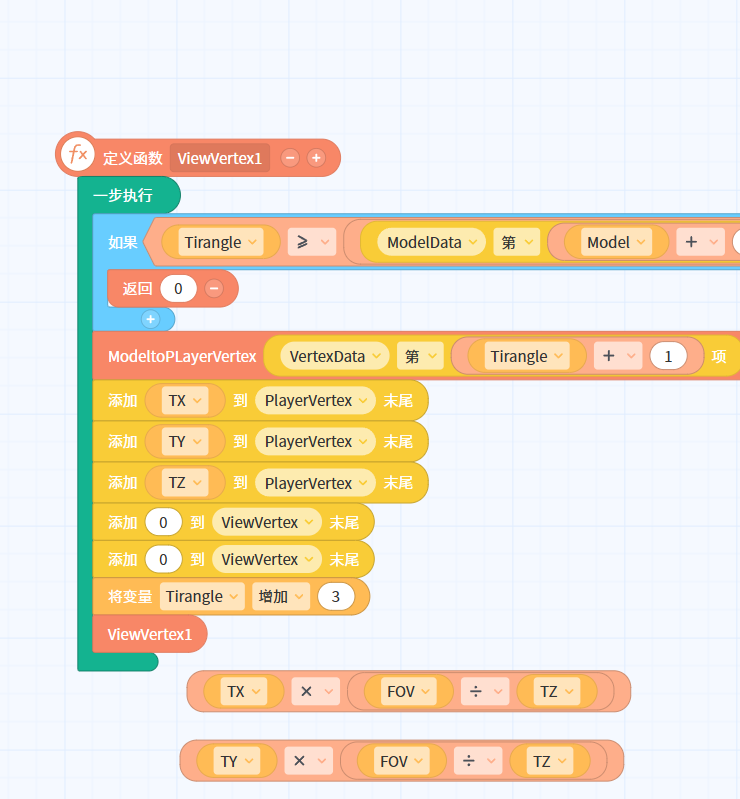
\includegraphics[width=0.5\textwidth]{assets/01/fire-2.png}
	
	此时运行
	
	
\includegraphics[width=0.5\textwidth]{assets/01/fire-3.png}
	
	一切正常,就说明这个代码不会参与到最终的渲染
	
	而会参与其他运算
	
	然后再去去除其他相关代码,直到无法去除
	
	最后根据之前的去除所得到的结论相结合,就可以知道这些代码是原来干什么的了
	
	如果你非常熟练编程,那你就不难发现这只不过是个递归
	
	\section{后记}
	\paragraph{编辑} 目前唯一编辑也是主笔:xiaole233 邮箱地址:xiao\_2010@outlook.com
	\paragraph{版权说明} 刊登的所有作品及文章均以取得原作者同意。\\ 
	猫站小报 第一期  © 2025 by 小报编辑部 is licensed under CC BY 4.0.\\ To view a copy of this license, visit https://creativecommons.org/licenses/by/4.0/
	
\end{document}